\chapter{System Description}\label{chap:sys_description}
The present chapter covers the system design including specific solutions that have been chosen for the realization of the SmartNotes application. The system concept, introduced in Chapter~\ref{chap:concept}, will become extended by describing certain elements of implementation and problems found during the development process. This should allow the reader to have a deeper view of the SmartNotes application, including the functions that it offers as well as the platform that it runs on.
\section{Google App Engine platform}\label{sec:gae}
Google App Engine seems to be an outstanding development platform. For all the reasons mentioned in~\ref{sec:gae_general}, it has been decided to be used as the main platform for SmartNotes as the one preceding any other hosting services. Besides, GAE appears to be highly competitive in terms of cost calculations, which are described in Section~\ref{subsec:gae_calculations}. After registering the application with a unique name, it can be easily uploaded to Google and after a few seconds it is accessible to its users.
 
As stressed in Section~\ref{subsec:sync_scenarios}, synchronization scenarios use the client-server architecture. When running on GAE platform, which is, as mentioned in~\ref{sec:gae_general}, a distributed vault-tolerant infrastructure, two subsequent request may be served by different machines located in separate data centres. Thus, in the addressing scope, the application can still be treated as a centralized server. In case the application requires state awareness, it is the developer's role to make it so; otherwise, the fact that the application is served from multiple machines is completely transparent from the functional point of view.
 
SmartNotes uses only some of the components supported by GAE and the ones which make a part of the SmartNotes application with relation with other third-party elements are presented in Figure~\ref{fig:smartnotes_components}. This is especially important as it presents all the application top level components together with marked interfaces between the particular functional blocks. This particular diagram strongly corresponds with the diagram from Figure~\ref{fig:ismartnotes_smartnotes}, which in a more general way presents the cooperation of SmartNotes and iSmartNotes with differentiated roles of the administrator and the user.
 
The most complicated structure is the one of the SmartNotes component, which is marked as an individual system. It does not require the iSmartNotes to realize its functionality. For this reason, the SmartNotes component could work with any kind of client application using the interface that the tool provides, or the interface of Mercurial HTTP chains of requests and responses that needed a back-end redesign to accommodate conditions set by GAE. The issues related to the cooperation of Mercurial and GAE are the topic of Section~\ref{sec:hg_on_gae}.
 
Furthermore, SmartNotes uses three additional interfaces which are used to interconnect the Google App Engine component with Mercurial adopted to run on GAE, as well as separately, admin and user interfaces provided by SmartNotes. Each of the three components is connected in a different way. Whereas the webapp framework has a low Python overhead as mentioned in Section~\ref{subsec:webapp} and was chosen to serve the connection between the Mercurial and the Google App Engine component, for performance reasons, it is Django which is the most optimal choice considering building of nontrivial web-based functionality for reasons mentioned in Section~\ref{subsec:django}. The remaining two elements used by the GAE subsystem are the Google Account and the Datastore. The role of the first one has been presented in detail while discussing the iSmartNotes activation process in Section~\ref{subsec:ismartnotes_activation}. Some of the Datastore details will be covered in Section~\ref{sec:hg_on_gae}.
\begin{figure}[ht]
\begin{center}
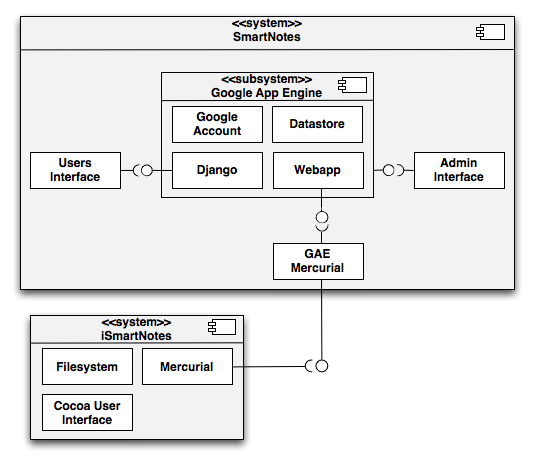
\includegraphics[scale=0.6]{charts/smartnotes_componets.pdf}
\caption{The components diagram of the SmartNotes application with marked interfaces between the functional blocks.}
\label{fig:smartnotes_components}
\end{center}
\end{figure}
 
The second independent system is the iSmartNotes component, which remains independent until the user decides to activate it to use the synchronization feature. For this purpose, it requires a Mercurial server to interact with. The iSmartNotes, as presented in Figure~\ref{fig:smartnotes_components}, is build with three components. Firstly, the file system of the client's operating system which is the classical space where VCS's allocate their repositories. Secondly, it is the Mercurial VCS, which on the client site does not require any modifications. %Finally, the Cocoa user interface, discussed in Section~\ref{sec:cocoa}.
 
\subsection{Financial calculations}\label{subsec:gae_calculations}
The role of this section is to introduce basic calculations that should give the reader a general experience of what resources will be used by the application with the connection to the billing rates set by Google. In the next step, these values will be used to predict the size order for the monthly cost of running the application per one million of SmartNotes users. This should help to indicate system elements that generate the highest price of resource usage, which in the end allows for concentrating on optimization within the specific area.
 
Calculations presented below aim to predict the theoretical monthly cost of running SmartNotes applications for one million of users with unit price detailed in Table~\ref{tab:gae_cost}. Each of resources will become briefly introduced with a short explanation of the assumptions taken. The outcome of these considerations is illustrated in Figure~\ref{tab:gae_cost}.
\begin{table}[h]
\centering
\caption{Google App Engine billing rates on September 2009.}
\label{tab:gae_cost}
\begin{tabular}{|l|l|l|} \hline \hline
\textbf{Resource} & \textbf{Unit} & \textbf{Unit cost} \\ \hline \hline
Outgoing Bandwidth & Gigabytes & \$0.12 \\ \hline
Incoming Bandwidth & Gigabytes & \$0.10 \\ \hline
CPU Time & CPU hours & \$0.10 \\ \hline
Stored Data & Gigabytes per Day & \$0.005 \\ \hline
Recipients Emailed & Recipients & \$0.0001\\ \hline \hline
\end{tabular}
\end{table}
 
Resource usage to price calculations:
\begin{itemize}
\item{\textbf{Outgoing Bandwidth}. This value represents a summarized amount of data send from the server to the users, which normally includes html, css, java script and graphic files as the standard web pages components. In hte classical case, a total size of a web page verges on \mbox{70--150KB}, which with compression can reduce it by a factor of about 40\%. In case of SmartNotes application the content sent between the server and iSmartNotes are the changesets. It was assumed that the size of an average downstream changeset won't exceed 2KB. It is smaller from the upstream changeset as not all server responses contain a changeset. A changset is sent only if there is a need for it, i.e. when the application encounters differences requiring synchronization.  
 
The next assumption regards the activity of users. As stated in the beginning, the calculations are done for one million of users. Additionally, there is a strong group of active users, which - translated into numbers - would mean that ca. 80\% of users generate four editing actions. This, accordingly to the synchronization scenario from Figure~\ref{fig:seq_commit}, might require sending the data from and to the server.  For this reason the bandwidth calculations for incoming and outgoing traffic use the same number of requests, which all in all leads to the fallowing numbers:
 
$Outgoing\ Bandwidth =  80\% \cdot 1,000,000\ users \cdot 4\ requests\ per\ user \cdot$\\ \hspace*{37mm} $2KB\ per\ request \cdot 30\ days \approx \textbf{183GB\ per\ month}$ \\
$Outgoing\ Bandwidth\ Cost = 183GB\ per\ month \cdot \$0.12\ per\ GB \approx \textbf{\$22 per\ month}$ }
 
\item{\textbf{Incoming Bandwidth}. In this case the same number of requests will be used just as in the case of the outgoing bandwidth. That is 3,200,000 of requests per day and it will be used as the basic parameter in all of the calculations mentioned below.
 
The size of a single request will be double the value taken when calculating the outgoing bandwidth. This is caused when each of the operations done by the use of iSmartNotes requires a changeset to be sent over. The remaining part of calculations regarding the incoming bandwidth follows the numbers which were used for the outgoing bandwidth:
 
$Incoming\ Bandwidth =  3,200,000\ requests\ per\ day \cdot 4KB\ per\ request \cdot 30\ days$\\ \hspace*{33mm} $\approx \textbf{366GB\ per\ month}$ \\
$Incoming\ Bandwidth\ Cost = 366GB\ per\ month \cdot \$0.1\ per\ GB \approx \textbf{\$37 per\ month}$ }
 
\item{\textbf{CPU Time}. This calculation was done by checking the average time when the CPU was idle while serving a single request. As mentioned in Section~\ref{subsec:webapp}, it has lower Python overhead and it was chosen over the Django framework for performance reasons. This, in consequence, allowed to reduce the CPU time parameter. Due to the fact that all requests require the CPU time, the base number of 3,200,000 requests per day is multiplied by two for upstream and downstream requests. Turning that into numbers gives:
 
$CPU\ Time =  3,200,000\ requests\ per\ day \cdot 2 \cdot 0.02\ seconds\ per\ request \cdot 30\ days$\\ \hspace*{17mm} $\approx \textbf{1067\ hours\ per\ month}$ \\
$CPU\ Time\ Cost = 1067\ hours\ per\ month \cdot \$0.1\ per\ hour \approx \textbf{\$107 per\ month}$}
 
\item{\textbf{Stored Data}. To help imagine the storage space needed for an average notes repository, it seems worth assuming that the popular collection of stories called "Winnie-the-Pooh" contains about 4,000 lines and its size in plain text without graphics is about 150KB. When using Version Control Systems it should be remembered, as it was mentioned in Section~\ref{subsec:hg}, that these systems consume additional disc space. The fudge factor saying how may times the final repository size will exceed its base content size is about 3 to 4 times, which depends on how many files are stored in that repository and how frequent the changes are. Altogether, assuming a size of 1MB for user repository seems to be reasonable and will make the calculations simple.
 
$Stored\ Data =  1,000,000\ users\cdot 1MB\ per user \cdot 1\ month \approx \textbf{977GB\ per\ month}$ \\
$Stored\ Data\ Cost = 977GB\ per\ month \cdot \$0.15\ per\ GB\ per\ month \approx \textbf{\$146 per\ month}$}
 
\item{\textbf{Mail}. In case of the iSmartNotes activation, there is no need to send mails to users like in the case of a classical account creation, as was discussed in Section~\ref{subsec:ismartnotes_activation}. On the other hand, e-mail remains a very effective way to communicate with users. Although there are other possibilities like twitter\footnote{Twitter is an micro-blogging application allowing to share ideas and live-stream information in the macro scale by the use of Internet.}, placing information on a web page or displaying dialog windows from the application, mailing users with the information remains a more solid and professional attempt. For that reason, it seems to be worth taking mailing service into account for keeping the users updated just as for sending invitations to potential new users. The additional 20\% of mails send is reserved just for that purpose --- allowing satisfied users to share the information about SmartNotes with their contacts.
 
$Mail =  1,000,000\ users\cdot (1 + 20\%) = \textbf{1,200,000\ mails\ per\ month}$ \\
$Mail\ Cost = 1,200,000\ mails\ per\ month \cdot \$0.0001\ per\ mail = \textbf{\$120 per\ month}$}
\end{itemize}
 
This altogether encloses ca. \$312 without mailing and about \$432 with mailing service. Beside the above, the application may use the free quota up to limits shown in Table~\ref{tab:gae_free}. The free quota resources should allow to reach a rate of 5 million page views per month, which could be used to serve the SmartNotes homepage or as a backup resource for the application.
\begin{table}[h]
\centering
\caption{Google App Engine free quota limitations on September 2009.}
\label{tab:gae_free}
\begin{tabular}{|l|l|} \hline \hline
\textbf{Resource} & \textbf{Daily Limit} \\ \hline \hline
Outgoing Bandwidth & 1 Gigabyte \\ \hline
Incoming Bandwidth & 1 Gigabyte \\ \hline
CPU Time & 6.5 CPU hours \\ \hline
Stored Data & 1 Gigabyte \\ \hline
Recipients Emailed & 2000 \\ \hline \hline
\end{tabular}
\end{table}
 
The above figures could be compared to popular hosting services like Rackspace or Amazon Web Services that offer the same resources for prices collated in Table~\ref{tab:services_price_compare}.
Some services like Joyent or Rackspace use another pricing strategy by using base service price with predefined resources and allowing users to extend it by ordering additional resources. Because of this, it becomes difficult to objectively compare resource prices in separate; hence it is more accurate to concentrate on the vales presented in Table~\ref{tab:services_price_compare} \emph{Summary} rows.   
 
Disregarding pricing differences it should be stressed that Google App Engine is not only a hosting service but also exposes for wide use Google infrastructure components that were mentioned in Section~\ref{sec:gae_general}. Furthermore, developers deciding to use Google App Engine gain access to a bunch of useful API's such as Memcache or URLfetch. Finally, the dashboard not only gives a clear view on the application status but also allows to flexibly control the expanses as well as to set a daily budget eligible for change anytime during the day. When certain capital becomes unused, it becomes available in the next days. On the other hand, applications using Google App Engine are protected from running out of resources by load peaks\footnote{This effect has a popular name - applications become \emph{slashdoted}, which might be the result of placing a link to an application on a highly popular social web services like \url{slashdot.org} from which the effect takes name; alternatively, it becomes a target of malicious scripts or load testing programs.}. For all those reasons, Google App Engine seems to be not only the most developer-friendly and flexible platform, but also offers a highly competitive pricing policy.   
 
\begin{table}[h]
\centering
\caption{SmartNotes resource prices among different hosting providers.}
\caption*{ $^{*}$ These prices could not be listed as some services use predefined resource sets and allow to buy extra resources.\\
 $^{**}$ These prices were calculated by using extra bandwidth and CPU time as mailing is not separately billed by the services. That was done by taking the following constants: $Average\ Mail\ Size = 100KB$, $CPU\ Time\ per\ 100\ Mails = 0.01s$\\
 $^{***}$ These prices do not include mail service as it is supplementary for SmartNotes application.}
\label{tab:services_price_compare}
\begin{tabular}{|l|l|l|l|l|} \cline{3-5}
                              \multicolumn{2}{c|}{}       &\multicolumn{3}{c|}{\textbf{Resource Price by Service}} \\ \hline \hline
\textbf{Resource} &\textbf{Quantity} &\textbf{Google}        &\textbf{Amazon}         &\textbf{Rackspace} \\
                                               &                                             &\textbf{App Engine} &\textbf{Web Services} &  \\ \hline \hline
Bandwidth &550 Gigabytes &\textbf{\$59} &\$68 &\$69 \\ \hline
CPU Time &1067 Hours &\$107 &\$170 &\textbf{\$48}\\ \hline
Stored Data &977 Gigabytes &\$146 & \$216 &\$146 \\ \hline
Mail &1,200,000 Mails &\$120 &\textbf{\$20}$^{**}$ &\$26$^{**}$ \\ \hline \hline
\multicolumn{2}{|c|}{\textbf{Summary}} &\$432 &\$474 &\$100$^{*}$+\$289=\textbf{\$389}\\
\multicolumn{2}{|c|}{} &\textbf{\$312}$^{***}$ &\$454$^{***}$ &\$100+\$263=\$363$^{***}$\\ \hline \hline
\end{tabular}
\end{table}
 
Charts presented in Figure~\ref{fig:gae_cost} may be used to indicate the resource that the usage uees most. Considering the visualized proportion, it is clear that the bandwidth is not as problematic as the storage, mailing or the CPU time. When mailing service remains supplementary by optimizing the storage, the price becomes reduced. In order to achieve that, one of possible ways is to reduce the history size that is stored with the notes repository. By creating a queue task\footnote{This is one of the Google App Engine features that was introduced in Section~\ref{sec:gae_general} that allows to run tasks in background when the system is not busy.} that would reorganize the SmartNote repositories to store only 20 most recent changesets, the repository size might get reduced up to 50\%.     
 
\begin{figure}[ht]
  \begin{center}
    \subfigure[\textbf{Without mailing service}.]{\label{fig:gae_cost_without_mail}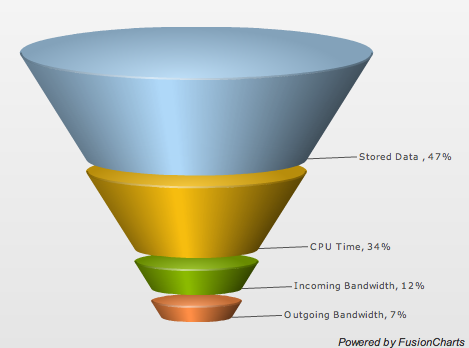
\includegraphics[scale=0.45]{img/price_div.png}}
    \subfigure[\textbf{With mailing service}.]{\label{fig:gae_cost_with_mail}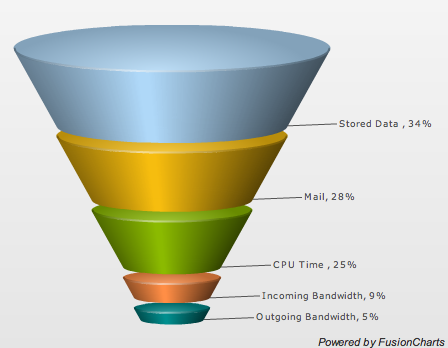
\includegraphics[scale=0.45]{img/price_div_mail.png}}
  \end{center}
  \caption{Simulated monthly cost division of resources expected to be used by one million of SmartNotes users on Google App Engine.}
  \label{fig:gae_cost}
\end{figure}
 
\subsection{Scalability}\label{subsec:scalability_on_gae}
Scalability was one of the main design concerns of the presented project. As mentioned in Chapter~\ref{sec:Introduction}, the SmartNotes application was meant to meet scalability requirements as well as to care for the best user experience. Additionally, the architecture should allow for a future development of flexibility. In the classical case, the applications may scale up to a relatively low level, however, a successful implementation of scalability patterns allows to shift this point further by keeping the cost growth linear depend on the served traffic. 
 
Identifying SmartNotes scalability barriers was the first essential step in the planning phase. Next, possible solutions were considered which finally allowed to take architectural decisions and start their implementation.  
\begin{itemize}
\item{Data retrieval. This superficially trivial problem becomes a true bottleneck for many systems aggregating data. In the most popular case, the time needed to retrieve certain data from the database is proportional to the amount of data stored. Scalable data retrieval model implies that the time needed to find and return data is proportional to the amount of queried data disregarding the number of data stored in database. Besides, the increased system load should have a minimum effect on the system performance, which requires the usage of a well prepared architecture and allows for flexible memory administration. All of these are requirements met by the BigTable, despite the fact that they are extremely difficult to achieve when a classical relational database is being used. Moreover, these systems are of great use when the data stored does not have the potential of a dramatic growth or can easily become partitioned, having a considerable impact on development process. 
 
In the case of SmartNotes, the data is organized in a structures defined by the Mercurial version control system. The data should become organized in a way that leaves access to the structures optimal and within the scope of a particular user. That is especially a matter of when the data is stored on multiple machines that can be possibly located in distant data centers. Minimizing this interoperation or ensuring constant duration is a serious scalability concern. As it was already identified by Google engineers, a solution is available. Placing related entities in structures called entity groups causes them to be stored close within the disc space, which results in less varied access time. By eliminating the fluctuations, data retrieval might deliver the same level of latency disregarding the total amount of stored data.}
\item{Bandwidth. This parameter may become crucial when the application bandwidth usage is significant. Once, due to the fact that it will cost twice when the maximum allowed link throughput might be reached. This, considered together with network latency fluctuations, motivate the minimizing of the size and number of transferred packages.
 
Effective usage of HTTP protocol was an important concern while choosing a Version Control System. Mercurial characteristics~\cite{google_hg_git_compare} were one of its greatest advantages. Basing on them, SmartNotes may form better bandwidth utilization by varying the synchronization changesets rate. Because of the fact that basic configuration was satisfied the limitations set by Google, no additional optimization techniques were used, an exception being the synchronization feature which was discussed in Section~\ref{subsec:sync_scenarios} while presenting synchronization scenarios on Figures~\ref{fig:seq_commit} and \ref{fig:seq_commit2}. On the other hand, it is important to clearly note that this issue is one of the system fundaments and deserves close attention during further development.}
\item{Framework. Referring to the notes made in Section~\ref{sec:scalability} regarding the scalability term, it is not a particular technology that makes the application scale well, neither it is easy to form general best practices for building web applications. Scalability becomes a part of application planning, therefore it depends strongly on the application characteristics. In effect of successfully implemented scalability patterns, the final result might be a \textit{"system that does not need to change when the size of the problem changes"}\cite{mike_malone_quote}.}  
\end{itemize}
 
With a view of all those aspects, the abovementioned framework choice is not the most crucial decision. On the other hand, a well structured framework can play a very important role in the development cycle. Once, it provides a frame for the application where the developer complements the parts that the application will use and twice, it often ships with functional blocks that are ready to be used in the application. Adding a clear structure and transparent documentation is what serves as the main decision criteria. In the case of SmartNotes, it was important to serve the Mercurial synchronization feature by a minimum Python overhead framework that would allow for extensive HTTP protocol control. The remaining functionality should be realized by an elastic framework that allows for rapid prototyping and that would care for the way the project is organized. This motivates the frameworks choice from Figure~\ref{fig:smartnotes_components}. They are what appeared to be the best choice for Python combined with the Google App Engine platform.   
 
\subsection{Security considerations}\label{subsec:security}
Security, just like scalability, are subjects of utmost importance especially for applications exposed to broad usage. Having that in mind, the following section aims to make the reader familiar with the main attempts used to secure the SmartNotes application. The weakest points of network applications are interfaces exposed to users or client applications. Therefore, security issues raised in this section will regard the components of interfaces that were presented in Figure~\ref{fig:smartnotes_components}. The list of security patterns is presented below:
\begin{itemize}
\item{SSL for all authenticated requests. By using this common technique all private data is exchanged between user and server using an encrypted connection. Therefore, while accessing the network, even traffic records will not allow for taking over credentials or any other private data from the SmartNotes users.
 
The above protection has become standard and most probably is the reason why Google decided to support it in the main configuration file. The basic form of \texttt{app.yaml} contains two sections. While the first one defines the application’s top level parameters like version, runtime or application identifier, the role of the second is allow for URL dispatching by defining regular expressions with actions that should become performed when an incoming URL matches a particular regular expression. One of the supported options is executed by key \texttt{secure} that is used in combination with one of three valid values \texttt{always}, \texttt{never} and \texttt{optional}. This parameter decides whether the request should become redirected to HTTP or HTTPS in the case of secure connection.}
 
\item{Secure Authentication. This element often is the key value for the security of the entire system. The way authentication parameters are created and restored should be measured in two scales. Firstly, it is designed with the user in mind, requiring two different and secure passwords the system gains for security (yet, this procedure may discourage a number of potential users). Secondly, application designers should treat seriously all security aspects and be able to find a middle ground between the reasonable level of security and user friendliness.
 
Because Google is a huge international company with a constantly increasing number of products gathering new users, it treats security aspects with high priority. Google account management allows for accessing multiple services simultaneously with the use of a single account, which makes it easy for users to examine new Google services and increases the importance of authentication. A malicious application that would gain the Google account credentials would give its author the right to access all of Google services using the stolen identity. This includes not only read access, but also full editing privileges allowing to modify or even delete its victim’s data. Being aware of this threat, Google created authentication systems that are well protected against all kinds of intruders.
 
While considering an authentication system for SmartNotes, it seemed that Google account is the best choice for the authentication service. Google has proven that users can rely on their products and additionally, it is authentication that is a part that the company prides itself in, which secures its future and allows for an easy integration in the application logic. This includes webapps just as the Django framework. If it is assumed that the dashboard functionality requires prior authentication, the specific part of configuration file might look as follows:
\lstset{language=Python,caption=Part of SmartNotes application configuration file app.yaml.,label=code:app_yaml_secure,
basicstyle=\scriptsize,         % the size of the fonts that are used for the code
showspaces=false,               % show spaces adding particular underscores
showstringspaces=false,         % underline spaces within strings
showtabs=false,                 % show tabs within strings adding particular underscores
tabsize=2,                    % sets default tabsize to 2 spaces
captionpos=b,                   % sets the caption-position to bottom
breaklines=true,                % sets automatic line breaking
breakatwhitespace=false,        % sets if automatic breaks should only happen at whitespace
escapeinside={\%*}{*)}          % if you want to add a comment within your code
}
\lstinputlisting{src/samples/app_yaml_secure.yaml}
As it was mentioned in previous points, by the use of a regular expression the developer is able to define an action with additional parameters to serve a particular group of requests. In this case, URLs \url{/dashboard/}, \url{/en/dashboard/} or \url{/es/dashboard/get_activation_key/} match the URL pattern from Listing~\ref{code:app_yaml_secure} and become served by \texttt{main.py} script. When the dispatcher becomes queried with one of these URLs, it first checks whether the user is authenticated; if so, it serves the request using HTTPS, otherwise, the user becomes redirected to a standard Google account login page and after successfully passing username and password controls they become redirected back to the dashboard.}
\item{Protecting user identity. All patterns described before help to fulfill that role. This point addresses the same problem but from some slightly different view, which relates to two issues that needed to become solved to realize the SmartNotes functionality.
 
The first issue regards the usage of a user identifier for personalized requests. The technique is used to minimize the volume of data stored in a single session as well as session queries. However, using a plain user identifier in the URL is a serious danger to security. Any logged in user may try their luck to check what happens when he changes to i.e. \texttt{userid} parameter in the browser URL bar. With a number of trials their curiosity might become rewarded in uncontrolled access to another user’s data, which is also a prime example for the statement that security remains developer’s responsibility without depending on security of the tools he uses. When choosing this technique, user identifiers should be protected by a hashing function that makes it relatively harder to guess the identifier of another user. However, the latter is still possible and in order to ensure security, the user with a given identity should have a cookie with a random value set from the domain. Yet, this amounts exactly to the definition of how a session mechanism works, which in consequence leaves the optimal solution of using the session itself to authorize requests. Therefore, SmartNotes uses the session for authenticating and building personalized web pages.   
 
The second problem arises with the will of making a SmartNotes interface that would work from outside the web browser. This requires also the authentication of the user as well as providing user-specific settings. When using a non-browser interface, the authentication mechanism used at Google does not seem to be suitable at all. Therefore, the fundamental idea was to rely on the Google account and take profit from all the abovementioned aspects without prompting SmartNotes users for their Google account username and password. The optimal solution was to use an activation key that would store the credentials and user settings so that only users would log in to SmartNotes with their Google account by clicking on the right link, generating their activation key and coping it to all iSmartNotes clients they use. Yet, data stored in the activation key would become encrypted using a symmetric encryption algorithm, which makes it relatively simple for the activation key to become as compact as possible. The algorithm should allow for future data retrieval without relying on any kind of passwords which amount to week protection. Thus, the solution is to generate a cryptographically strong pair of login and password that would uniquely identify the Google account user object.
Indeed, uniqueness is strongly desired not to let any two users have same pair of login and password, therefore using the table primary key as login and generating random password seems to be the solution for the problem. The part of code realizing this task is shown in Listing~\ref{code:user_gen_random}. Presented \texttt{get\_activation\_key} method returns a encoded form of activation key. It checks if the user has generated the activation key: if so, it uses the generated password, otherwise, the password becomes generated using \texttt{\_\_gen\_random} method. The latter is a string consisting of thirty characters which are taken randomly from a group that is built of digits, small and capital ascii letters and punctuation symbols. By using a group of $94$ different symbols instead of $62$ symbols, including only digits and letters, it is possible to reach a number of $94^{30}$ combinations which is more than $250000$ times greater when using a group of $62$ symbols.
\lstset{language=Python,caption=Part of Python User class used to model SmartNotes users.,label=code:user_gen_random,
basicstyle=\scriptsize,         % the size of the fonts that are used for the code
showspaces=false,               % show spaces adding particular underscores
showstringspaces=false,         % underline spaces within strings
showtabs=false,                 % show tabs within strings adding particular underscores
tabsize=2,                    % sets default tabsize to 2 spaces
captionpos=b,                   % sets the caption-position to bottom
breaklines=true,                % sets automatic line breaking
breakatwhitespace=false,        % sets if automatic breaks should only happen at whitespace
escapeinside={\%*}{*)}          % if you want to add a comment within your code
}
\lstinputlisting{src/samples/user_gen_random.py}
The activation code structure which was presented in Figure~\ref{fig:activation_key} becomes serialized using fast and secure \texttt{cPickle}\footnote{\texttt{Pickle} is a Python module implementing algorithm for serialization and de-serialization of Python objects. Other module called \texttt{cPickle} performs the same operation but it has been implemented with performance as a top priority allowing for up $1000$ times faster operations. That might be compared with \texttt{marshal} a module with great performance that is internally used by a Python interpreter to perform serialization and de-serialization, however it was never intended to perform security checks. Therefore it s not advisable to use it with data from any unreliable source.} module to become later encrypted using \texttt{base64}\footnote{Encoding \texttt{base64} takes its name from the number of $64$ printable characters it uses as base group in the encoding process. It has been used to encode binary content into 7-bit encoding for systems that have not supported 8-bit encoding. Although it was not created as a strong encrypting mechanism, it can be used to generate randomly looking sequences that can be later easily retrieved encapsulating the binary data.} encoding. The returned value is a randomly looking string that can be copied and pasted to the client application. It allows for saving the user’s time to write his credentials and settings in each of the client applications they decide to use.}
\end{itemize}
 
Summing up the above techniques, the main risk regarding SmartNotes is due to the interfaces it exposes. The presented ideas become implemented giving SmartNotes users privacy and data protection measures.
\subsection{Limitations}\label{subsec:limitations}
Google App Engine with Python runtime, which has been introduced in Section~\ref{sec:gae_general} and discussed in more detail in prior subsections, will become analyzed for potential limitations that SmartNotes development might find on its way. Findings are presented below in a list ordered by problem importance:
\begin{itemize}
\item{Libraries restrictions. Mainly for security reasons Google decided to restrict usage of any C extensions or other code that requires compilation or access to system sockets. Also, process and thread spawning is banned by Google and their usage results in raising exceptions. Although it might at first glance discourage some developers, it does not only care for security of Google servers but also for other developers applications. It looks as the only possible way that Google could expose their infrastructure for wide usage. This inconvenience is rewarded by rich functionality and competitive pricing policy. However, it is not the only question if a given application can incorporate these restrictions; also, the risk should be calculated as in the future it will not be allowed to use new third-party software which violates the conditions set by Google.}
 
\item{Framework boundaries and code transplantability. In case of webapp just as any other web framework known to the author, the developer does not have the possibility to freely migrate the code of an application between frameworks. Currently it is also impossible that the frameworks could cooperate by communicating with each using some other medium than the HTTP protocol. Altogether, the choice of framework binds the developer to that particular framework. This, in turn, also regards the code that becomes created, making it time consuming to transform and use it with another framework even if it realizes simple functionality.}
 
\item{Level of Google dependance. What was considered as Google App Engine’s greatest strength might be also taken as its biggest weakness. When a part of Google infrastructure fails, it may occur that it also affects App Engine as well since certain services are strongly related. The level of dependence in the case of Google App Engine is significant when it comes to the terms of service or the changes that Google can introduce in the future releases of its Software Development Kit.}
 
\item{Different runtimes cooperation. Currently, Google provides two runtime environments: Python and Java. Because the language support in the case of GAE is pluggable, it can be expected that this group will continue to expand. However, currently the only possibility to make use of different runtimes is to register them as separate applications that will have an individual datastore, use different machines and become billed and monitored separately. This kind of separation might be desirable in many cases but the lack of option allowing to use them in closer cooperation is considered as limitation.}
 
\item{Building RESTful\footnote{REST is an acronym for \textit{Representational State Transfer} and forms a scheme for writing web services. RESTful web services are more dynamic and powerful than the classic case of CGI web services as they make extensive use  methods provided by the HTTP protocol. For those reasons, among others, REST become popular and is used by such a solutions like Yahoo! Web Services.} applications. This particular kind of tools has become standard for writing web applications and is especially widely used in web services. Their biggest advantage is the clarity of its fundaments and as a matter of fact, due to its standard, it is easier to write functionality on top of it. When using Google App Engine, REST may be implemented by using more complex frameworks like Django or Pylons, which might be considered as a limitation, basing on the simple routing mechanism that does not differentiate requests on type of HTTP request, being the fundament for RESTful applications.}
\end{itemize}
All in all, the abovementioned limitations are problematic yet none of them is considered as a real barrier for SmartNotes development. The top three are of main concern as they have had the greatest impact on SmartNotes.
 
\section{Mercurial on Google App Engine}\label{sec:hg_on_gae}
Mercurial, a Version Control System which was generally introduced in Section~\ref{subsec:hg} realizes a fundamental role in the SmartNotes application. It is used, as shown in Figure~\ref{fig:smartnotes_components}, to ensure cooperation between the client iSmartNotes application with the SmartNotes server running on Google App Engine. Moreover it also significantly eases the implementing of notes synchronization what is one of the most important SmartNotes functionality's. The reader will become familiarized with some of the main development difficulties as well as have a deeper view in certain Mercurial internal mechanisms. Staring with the Mercurial base data structure, this section will cover its realization and will finish with the relevant Mercurial code modifications needed to let it run on GAE.
 
When any change tracked by Mercurial takes place, it uses \texttt{filelog} as the most fundamental structure to store all relevant data. Each of \texttt{filelog} entries stores enough data to reconstruct a single revision of a file. Using hash functions\footnote{Algorithms like \texttt{MD5} or \texttt{SHA1} can with high confidence identify data content by returning respectively 128-bit and 160-bit long checksums.} Mercurial does not only differentiate changesets, but also cares for data integrity. It should be noted that Mercurial utilizes the mechanism of cumulative deltas with the 'base' \texttt{filelog} revision storing the entire content and 'delta' revisions storing only the differences between it and the prior committed revision. When Mercurial notices that the cumulative size of deltas has elapsed just as the size of its base version, a new 'base' of that file becomes added to \texttt{filelog}. That way access to particular revisions is much faster requiring only to find the closest 'base' and read all the deltas against the desired revision number. Another data structure that is being utilized by Mercurial is called \texttt{manifest} and it allows to connect the information stored in \texttt{filelogs} with a particular changeset. It contains such information like a list of files present in a changeset with their control sequences. Therefore, the \texttt{changelog} is responsible for saving all the changeset metadata like the author, commit comment or date that the changeset became created. In order to illustrate the inner relationship between this structures, Figure~\ref{fig:hg_revlog} presents them in a hierarchy with the most general \texttt{manifest} at the top. Both \texttt{manifest} and \texttt{filelog} contain references to each other in scope of the corresponding revision, which helps Mercurial perform reverse lookup using the revision number.
\begin{figure}[ht]
\begin{center}
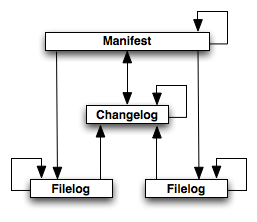
\includegraphics[scale=0.6]{charts/hg_revlog.pdf}
\caption{The Mercurial revlog data structures.}
\label{fig:hg_revlog}
\end{center}
\end{figure}
With that in mind it is obvious why all structures presented in Figure~\ref{fig:hg_revlog} contain a self-referential relation to the corresponding 'base' revision. Additionally, as a single revision can accumulate changes from more than a single file, there is possibility that more than one \texttt{filelog} points to a \texttt{changeset} entity. All of the structures become mapped from file-based storage into Google datastore. This was not only necessary to build the SmartNotes application, as none of the applications running on GAE can create or delete files, but it also helps to monitor system reaction on increased usage. Moreover, it is extremely important to use reliable tools allowing to monitor system status and provide a basis for performance and scalability analyses. Building it on file storage level could be very problematic especially in a distributed environment. Using an abstract layer, like the one provided by Google datastore, makes this task easier. Also, most of the desired metrics can be obtained directly from the GAE dashboard. Taking advantage of those tools\footnote{about those tools and Jmitter} the reader will be presented  the final results of Smartnotes in Section~\ref{sec:performance}.
 
Breaking the primary concept of storage in order to take advantage of Google, datastore was required not only to re-consider data structures used by Mercurial and write appropriate models replacing them, but also to use datastore for all kinds of storage purposes including the repository tree. This change should not, however, influence the cooperation with native Merurial modules methods on the client side. The compatibility is important because it makes it possible to complete the integration of SmartNotes with other applications that already use Mercurial version control, the latter concerning mainly the client-server interface that is marked in Figure~\ref{fig:smartnotes_components}. A great help with that task was the project of Jun Mukai available on \url{http://hg-repos.appspot.com} which by Mercurial code modifications provides a code hosting service on Google App Engine. The majority of concepts used by the SmartNotes server side of Mercurial interface were inspired by that project. The Listng~\ref{code:hg_gae_models_1} presents the \texttt{Repository} class construction with joint datastore kind together with \texttt{User} kind named \texttt{RepositoryUser}. This way, a many-to-many relation between those two models can be established and it allows to retrieve each repository and user data separately; additionally, when needed, it can also be used to get related objects. More specifically, by following the example, users having access to particular ones, are returned as a \texttt{list} of \texttt{User} objects by simply calling \texttt{repository\_instance.users}.  
\lstset{language=Python,caption=Simplified Repository model with the many-to-many relation.,label=code:hg_gae_models_1,
basicstyle=\scriptsize,         % the size of the fonts that are used for the code
showspaces=false,               % show spaces adding particular underscores
showstringspaces=false,         % underline spaces within strings
showtabs=false,                 % show tabs within strings adding particular underscores
tabsize=2,                    % sets default tabsize to 2 spaces
captionpos=b,                   % sets the caption-position to bottom
breaklines=true,                % sets automatic line breaking
breakatwhitespace=false,        % sets if automatic breaks should only happen at whitespace
escapeinside={\%*}{*)}          % if you want to add a comment within your code
}
\lstinputlisting{src/samples/hg_gae_models_1.py}
That is achieved by the reverse reference and the \texttt{collection\_name} parameter which does nothing else than set a suitable name for that relation. It is a common technique\footnote{Many-to-many relations are also used by legacy relational databases. From the programmer perspective it is only the API difference eg. Django assumes all fields are required by default and uses the \texttt{related\_name} parameter to give names for reverse relations.} allowing to form theoretically unlimited relations between datastore objects. Another interesting and also common data modeling pattern is illustrated in Listing~\ref{code:hg_gae_models_2}. Following the way Mercurial organizes his data two classes \texttt{ChangeLog} and \texttt{FileLog} were created to shore Mercurial data in the Google datastore.
\lstset{language=Python,caption=Two model classes being the functional equivalent of Mercurial structures.,label=code:hg_gae_models_2,
basicstyle=\scriptsize,         % the size of the fonts that are used for the code
showspaces=false,               % show spaces adding particular underscores
showstringspaces=false,         % underline spaces within strings
showtabs=false,                 % show tabs within strings adding particular underscores
tabsize=2,                    % sets default tabsize to 2 spaces
captionpos=b,                   % sets the caption-position to bottom
breaklines=true,                % sets automatic line breaking
breakatwhitespace=false,        % sets if automatic breaks should only happen at whitespace
escapeinside={\%*}{*)}          % if you want to add a comment within your code
}
\lstinputlisting{src/samples/hg_gae_models_2.py}
By separating the informations stored by those structures two significant advantages are reached:
\begin{itemize}
\item{Saving disk space. Using one-to-many relation helps to reduce disc usage by reducing redundant data, which means that there is no need to store informations grouped by \texttt{ChangeLog} with every file that the change regards. The idea is to store that data once and only refer to it from the \texttt{FileLog} objects.}
\item{Saving bandwidth. Assuming that the user is interested to get an overview of which files become changed on the turn on last two months, it would lead to bandwidth waste to respond with a all the data that has become changed during that time when the plain list of files with flags would be sufficient. Especially in the case of frequent and large changes that point has significant value also for the application performance.}
\end{itemize}
 
However, changing the data representation was not the only relevant change to make the Mercurial version control run on Google App Engine. It might be kind of obvious that all the parts responsible for reading or writing the data to Mercurial structures are required to be adapted to use the datastore API for those operations. Moreover, file representation was often changed to Python \texttt{StringIO} objects that provide file-like operations that can be performed on a string buffer. Altogether, porting Mercurial onto Google App Engine had the biggest significance for the SmartNotes application and was one of the most complex problems.      
 
%\section{Cocoa user interface}\label{sec:cocoa}
%\subsection{PyObj-C}
%\subsection{Interface project}
 
